\documentclass[12pt]{article}
\usepackage[utf8]{inputenc}
\usepackage{amsmath}
\usepackage{amsfonts}
\usepackage{amssymb}
\usepackage{graphicx}
\usepackage{float}
\usepackage{booktabs}

% --- Add these to mimic MS Word ---

% 1. Margins: Sets standard 1-inch margins on all sides
\usepackage[margin=1in]{geometry} 

% 2. Paragraphs: Removes the first-line indent and adds space between paragraphs
\usepackage{parskip} 

% 3. Line Spacing: Makes the lines slightly less cramped
\usepackage{setspace}
\setstretch{1.15} % 1.15 is MS Word's default. Use \onehalfspacing for 1.5 spacing.

\title{Assignment 4}
\author{Shapnil Das}
\begin{document}

\maketitle

\section{Question:}
In macroeconomics, we often debate whether a series is a Random Walk or just Very Persistent.
Simulate two variables for T = 150 observations:

1. Variable A (The Unit Root): A random walk with a drift of 0.2.

2. Variable B : A stationary AR(1) process with rho = 0.96 and a deterministic trend of 0.2t.

Run an Augmented Dickey-Fuller (ADF) test on both.
Did the ADF test correctly identify Variable B as stationary?
Use Monte-Carlo simulations to show why there is this debate.

\section{Solution:}
\subsection{ADF Test:}

We were provided instructions to simulate a Random walk with a drift process which can show
\textbf{Difference Stationarity} and a stationary AR(1) process with a deterministic trend which shows \textbf{Trend Stationarity}.

\begin{itemize}
    \item \textbf{The Unit Root: A random walk with a drift of $0.2$}
          \begin{equation}
              y_t = 0.2 + y_{t-1} + \varepsilon_t
          \end{equation}

          where $\varepsilon_t$ is a white noise error term.

          We can write this equation as:
          \begin{equation}
              y_t = 0.2t + \sum_{i=1}^{t} \varepsilon_i
          \end{equation}

    \item \textbf{ A stationary AR(1) process with $\rho = 0.96$ and a deterministic trend of $0.2t$}
          \[ x_t = 0.2t + \eta_t \]
          where \[\eta_t = 0.96\eta_{t-1} + \varepsilon_t \]
          and $\varepsilon_t$ is a white noise error term.
\end{itemize}

Theoretically, it can be hard to distinguish between a random walk with a drift and a Trend Stationary process with a deterministic trend with visualizations.


\includegraphics[width=\textwidth,scale=1.2]{./tsplot_hw4_1.png}


\includegraphics[width=\textwidth,scale=1.2]{./tsplot_hw4_2.png}

We can see that both the series have an upward trend and it is hard to visually identify which one is a random walk and which one is a stationary process with a deterministic trend.
So we need to perform an Augmented Dickey-Fuller (ADF) test to identify which one is a random walk and which one is a stationary process.
First we have to check for the number of lags in each variable. Using the vector autoregression varsoc command, we can identify the optimal number of lags for each variable.
The optimal lag is 1. So we run an ADF test with lags(1).



\begin{table}[H]
    \centering
    \renewcommand{\arraystretch}{1.2}
    \setlength{\tabcolsep}{12pt}
    \caption{ADF Test of Random walk with drift}
    \vspace{0.15cm}
    \begin{tabular}{lrrrr}
        \toprule
               & \textbf{Test}       & \multicolumn{3}{c}{\textbf{Dicky Fuller Critical Values}}                                \\
               & \textbf{Statistics} & \textbf{1\%}                                              & \textbf{5\%} & \textbf{10\%} \\
        \cmidrule(lr){2-5}
        $Z(t)$ & $-2.596$            & $-4.024$                                                  & $-3.444$     & $-3.144$      \\
        \bottomrule
        \addlinespace
        \multicolumn{5}{l}{\footnotesize MacKinnon approximate p-value for $Z(t) = 0.2820$.}
    \end{tabular}
    \label{tab:adf_test_booktabs}
\end{table}



The ADF test correctly identifies Variable A as a random walk with a drift and fails to reject the null hypothesis of a unit root.
The p-value is $0.2820$ which is greater than $0.05$, which means we fail to reject the null hypothesis of a unit root.



\begin{table}[H]
    \centering
    \renewcommand{\arraystretch}{1.2}
    \setlength{\tabcolsep}{12pt}
    \caption{ADF Test of AR (1) with $\rho = 0.96$ deterministic trend variable}
    \vspace{0.15cm}
    \begin{tabular}{lrrrr}
        \toprule
        \addlinespace
               & \textbf{Test}       & \multicolumn{3}{c}{\textbf{Dicky Fuller Critical Values}}                                \\
               & \textbf{Statistics} & \textbf{1\%}                                              & \textbf{5\%} & \textbf{10\%} \\
        \cmidrule(lr){2-5}
        $Z(t)$ & $-2.276$            & $-4.024$                                                  & $-3.444$     & $-3.144$      \\
        \bottomrule
        \addlinespace
        \multicolumn{5}{l}{\footnotesize MacKinnon approximate p-value for $Z(t) = 0.4475$.}
    \end{tabular}
    \label{tab:adf_test_ar1_booktabs}
\end{table}



Even though variable B is a stationary process, the ADF test fails to identify Variable B as a stationary process with a deterministic trend and fails to reject the null hypothesis of a unit root with a p-value of $0.4475$.

\subsection{Monte-Carlo Simulation:}

Earlier we have seen the ADF test fails to identify Variable B as a stationary process. To investigate why this happens we perform a Monte-Carlo Simulation
to do a Type-2 Error Power test to check how many times the ADF test do not reject the false null hypothesis of a unit root when the alternative hypothesis
is true and the series is actually stationary.

We use Stata's Program command to simulate 1000 estimation of ADF test statistics of 150 sample for variable A and Variable B.
Then we generate a dummy variable which calculates how many times the ADF test statistics is less than $-3.44$.Here the mean result is presented:



\begin{table}[H]
    \centering
    \renewcommand{\arraystretch}{1.4}
    \setlength{\tabcolsep}{18pt} % Generous breathing room    
    \caption{\textsc{Simulation Results:} Percentage of Rejection}
    \vspace{0.15cm}
    % The @{} removes the left and right outer padding for a flush look
    \begin{tabular}{@{} l c c c @{}}
        \toprule[1.5pt] % Thicker top border for framing
        \textbf{Data Generating Process} & \textbf{Observations} & \textbf{Mean} & \textbf{Std. Dev.} \\
        \midrule
        Random Walk with a drift         & $1000$                & $0.056$       & $0.230$            \\
        Trend Stationary ($\rho = 0.96$) & $1000$                & $0.099$       & $0.298$            \\
        \bottomrule[1.5pt] % Thicker bottom border for framing
    \end{tabular}
    \label{tab:beautiful_sim}
\end{table}



For the Random walk process we see that ADF test correctly identifies the unit root process almost $95\%$ times which aligns with the $95\%$ confidence interval at rejection rate $5\%$.
The Type-1 error of false rejection is only $5.6\%$.

For the stationary deterministic trend process,considering the rejection rate at $5\%$, almost $95\%$ of the time the ADF test should reject the null hypothesis of a unit root.
But we see the complete opposite result.The ADF test rejects the null hypothesis of unit root only $9.9\%$ times with a Type-2 error of almost $90\%$ resulting in a low statistical power test of Augmented Dickey-Fuller test.


\includegraphics[width=\textwidth,scale=1.2]{./hw4_kdensity.png}

\newpage
From the density plot,

the pink curve shows the unit root process with $95\%$ confidence interval at t-stat $-3.44$ at the vertical dotted black line.
The blue curve shows the stationary process with $\rho = 0.96$. Theoretically,the blue curve should fall completely to the left of the rejection area.Any area right to the dotted black line represents the Type-2 error for blue curve
.But the simulations exposes the huge Type-2 error of the blue curve and the unreliability of the ADF test to identify a stationary process when the process is near unit root process.


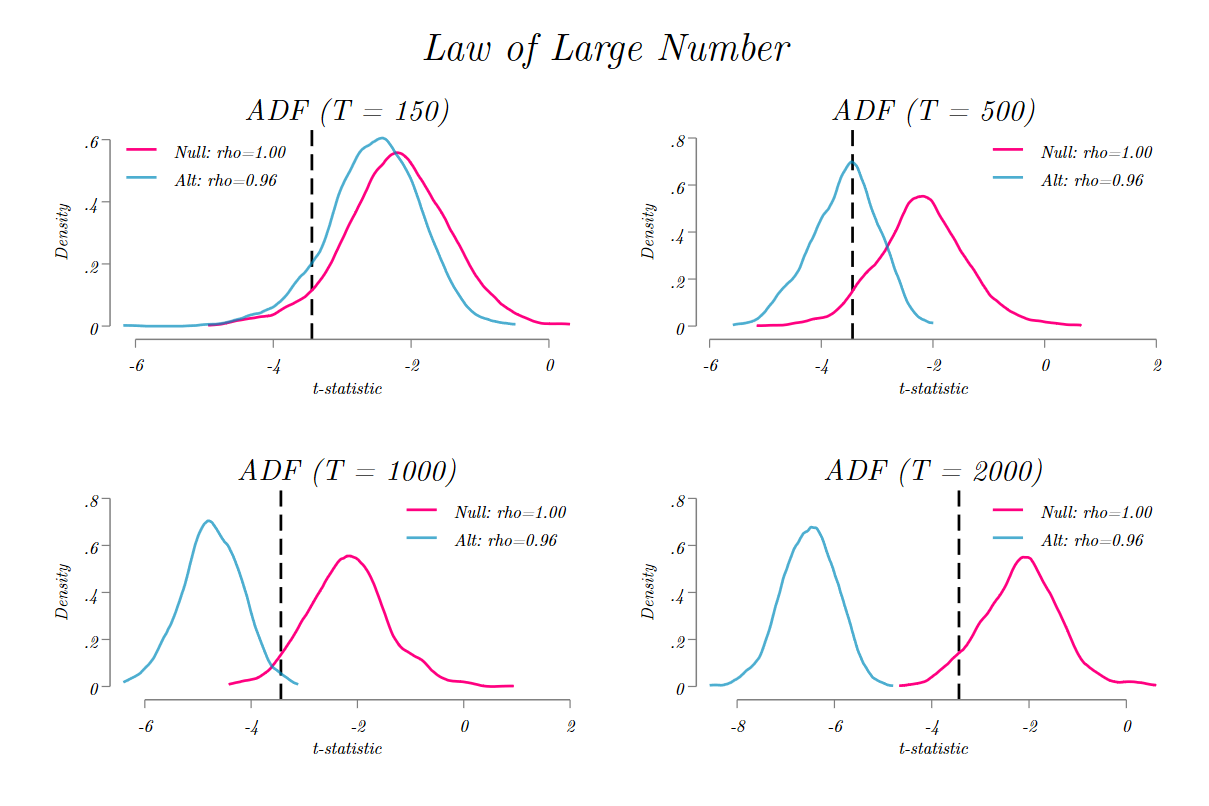
\includegraphics[width=\textwidth,scale=1.2]{./LLL.png}

The law of large numbers, a statistical property that says if we increase the number of samples, the estimated or simulated distribution will follow the true distribution of the population mean ,can help us to validate the low statistical power of ADF test.
we have taken 4 different sample sizes of $150, 500,1000,2000$ and simulated each sample $1000$ times to check the Law of large numbers property.
we can see from the stacked diagram that as we increase the sample from $150$ to $2000$ sequentially, the simulated ditribution moves to the left of the true ditribution resulting in lower Type-2 error
and higher power of the ADF test. So we can conclude that the ADF test has a low power to identify a stationary process when the process is near unit root process and we need to increase the sample size to increase the power of the ADF test
. This theory also validates the Monte-Carlo simulation results that we have obtained in this assignment as we have simulated each sample $1000$ times, with increased simulated sample the Monte-Carlo simulation can follow the true distribution of the population mean.
But in macroeconomics, we often have limited number of small sample that's why it's not easy to identify a stationary process with a deterministic trend when the process is near unit root process and this is why there is a debate in macroeconomics whether a series is a Random Walk or just Very Persistent.


\end{document}
